\documentclass[11pt]{article}
\usepackage[spanish]{babel}
\usepackage[utf8]{inputenc}

%Tipo de letra y color
\usepackage{FiraSans}                 % Fuente sans serif
\usepackage[T1]{fontenc}
\usepackage[usenames]{color}
\definecolor{ColorTitulo}{RGB}{169,50,38}

%Imágenes
\usepackage{graphicx}
\graphicspath{{img/}}
\usepackage{float}

%Matemáticas
\usepackage{amssymb}
\usepackage{amsmath}

%Código
\usepackage{listings}
\usepackage{xcolor}
\renewcommand{\lstlistingname}{Código}% Listing -> Código

\definecolor{dkgreen}{rgb}{0,0.6,0}
\definecolor{gray}{rgb}{0.5,0.5,0.5}
\definecolor{mauve}{rgb}{0.58,0,0.82}

%% \lstset{frame=tb,
%%   language=Sage,
%%   aboveskip=3mm,
%%   belowskip=3mm,
%%   showstringspaces=false,
%%   columns=flexible,
%%   basicstyle={\small\ttfamily},
%%   numbers=none,
%%   numberstyle=\tiny\color{gray},
%%   keywordstyle=\color{blue},
%%   commentstyle=\color{dkgreen},
%%   stringstyle=\color{mauve},
%%   breaklines=true,
%%   breakatwhitespace=true,
%%   tabsize=3
%% }

\definecolor{codegreen}{rgb}{0,0.6,0}
\definecolor{codegray}{rgb}{0.5,0.5,0.5}
\definecolor{codepurple}{rgb}{0.58,0,0.82}
\definecolor{backcolour}{rgb}{0.95,0.95,0.92}
 
\lstdefinestyle{mystyle}{
    backgroundcolor=\color{backcolour},   
    commentstyle=\color{codegreen},
    keywordstyle=\color{magenta},
    numberstyle=\tiny\color{codegray},
    stringstyle=\color{codepurple},
    basicstyle=\ttfamily\footnotesize,
    breakatwhitespace=false,         
    breaklines=true,                 
    captionpos=b,                    
    keepspaces=true,                 
    numbers=left,                    
    numbersep=5pt,                  
    showspaces=false,                
    showstringspaces=false,
    showtabs=false,                  
    tabsize=2
}
\lstset{style=mystyle}

%Márgenes
\usepackage[paper=portrait, pagesize]{typearea}
\usepackage{titlepic}
\setlength{\textwidth}{155mm}
\setlength{\textheight}{210mm}
\setlength{\oddsidemargin}{6mm}
\setlength{\evensidemargin}{28mm}
\setlength{\topmargin}{-10mm}

%Símbolo para las listas
\usepackage{listings}
\usepackage{enumerate}
\renewcommand{\labelitemi}{$\circ$}
\usepackage{enumitem}

%Encabezados y pies de página
\renewcommand{\thefootnote}{\roman{footnote}}
\usepackage{fancyhdr}
\pagestyle{fancy}
\fancyhf{}
%\rhead[R]{\MakeUppercase{\rightmark}}
\lhead[L]{\MakeUppercase{\textit{Curva Elíptica}}}
\fancyfoot[R]{\thepage}

\renewcommand{\sectionmark}[1]{
\markboth{#1}{}}
\renewcommand{\headrulewidth}{0pt} 

%Índice
\addtocontents{toc}{\hspace{-7.5mm} \textbf{Secciones}}
\addtocontents{toc}{\hfill \textbf{Página} \par}
\addtocontents{toc}{\vspace{-2mm} \hspace{-7.5mm} \hrule \par}

%Apéndices
\usepackage[toc,title,page]{appendix}

%Subíndices
\usepackage{amsmath}
\DeclareMathOperator{\Prob}{Prob}

\begin{document}

%%PORTADA%%
\begin{titlepage}
\centering
\vspace*{4.5cm}
\fontsize{30pt}{40pt}{\selectfont\sffamily{\textcolor{ColorTitulo}{Trabajo Teoría}}}\\
\vspace{5mm}
\fontsize{60pt}{50pt}{\selectfont\sffamily{\textcolor{ColorTitulo}{Curva Elíptica}}}
\vspace{1.5cm}

{\scshape\large \today \par}
\vspace{1cm}


\vspace*{\fill}
\raggedleft{Sofía Almeida Bruno\\
Pedro Manuel Flores Crespo\\
María Victoria Granados Pozo\\
\par}
\vspace*{-2cm}

\end{titlepage}

\thispagestyle{empty}
\tableofcontents

\newpage

\section{Introducción}

% Comentar que usaremos Sage en algún momento

\section{Curva Elíptica}
% Escribo esta sección inspirándome en el capítulo 2 de ``Elliptic Curves Number theory and cryptography'' y comparándo con otros artículos
Antes de entrar en cómo usar las curvas elípticas en criptografía debemos definirlas y estudiar su estructura de grupo.

Una curva elíptica será el conjunto de puntos que verifiquen la ecuación:
\[y^2 = x^3 + ax + b,\]
donde $a$ y $b$ son constantes y verifican $4a^3+27b \neq 0$\footnote{Imponemos esta condición para que la curva no presente raíces múltiples, que pueden dar problemas en la teoría general que expondremos. Se pueden tratar ambos casos de forma individual aunque nosotros no incluiremos estas excepciones en nuestro trabajo}. Esta ecuación es la \textbf{ecuación de Weierstrass} para curvas elípticas. Normalmente, $a, b, x, y$ toman valores en un cuerpo. Por ejemplo: los números reales $\mathbb{R}$, los números complejos $\mathbb{C}$, los números racionales $\mathbb{Q}$, un cuerpo finito $\mathbb{F}_p$ para un primo $p$ (este es el que se utiliza en criptografía habitualmente), un cuerpo finito $\mathbb{F}_q$ donde $q = p^k,$ $k \ge 0$, \dots

De forma general, consideramos un cuerpo $K$ y definimos la curva elíptica $E$ sobre él de la siguiente forma:
\[E = \{(x,y) \in K\times K : y^2 = x^3 + ax +b\} \cup \{\infty\}.
\]
El punto $\infty$ lo incluimos por definición. Lo podemos imaginar como un punto que se encuentra en la parte alta del eje y, pero también en la parte de abajo. Una línea que pase por este punto será una línea vertical, luego dos líneas verticales distintas coinciden en este punto.

Podemos usar Sage para visualizar algunos ejemplos de curvas elípticas. En el Código \ref{cod:EC} observamos la forma genérica de definir en Sage curvas elípticas.

%TODO: arreglar colores
% TODO: probar con language=Python
\begin{lstlisting}[label={cod:EC}, caption={Curva elíptica en Sage}, morekeywords={sage}]
sage:  E = EllipticCurve(K, [a, b]); E
Elliptic Curve defined by y^2  = x^3 + x + 3 over a field K
\end{lstlisting}

El Código \ref{cod:ej1} es el necesario para crear la curva con ecuación de WeiErstrass $y^2=x^3-1$.

\begin{lstlisting}[label={cod:ej1}, caption={Curva elíptica $y^2=x^3-x$}, morekeywords={sage}]
sage: E =  EllipticCurve(RR, [-1, 0]);
      plot(E, (-4, 3), color=hue(0.6))
\end{lstlisting}

Podemos observar la salida obtenida en la Figura \ref{fig:ej1}.

% Cuando terminemos de escribir ya reajustamos tamaño y posición de las figuras para que no queden espacios en blanco
\begin{figure}[H]
    \centering
    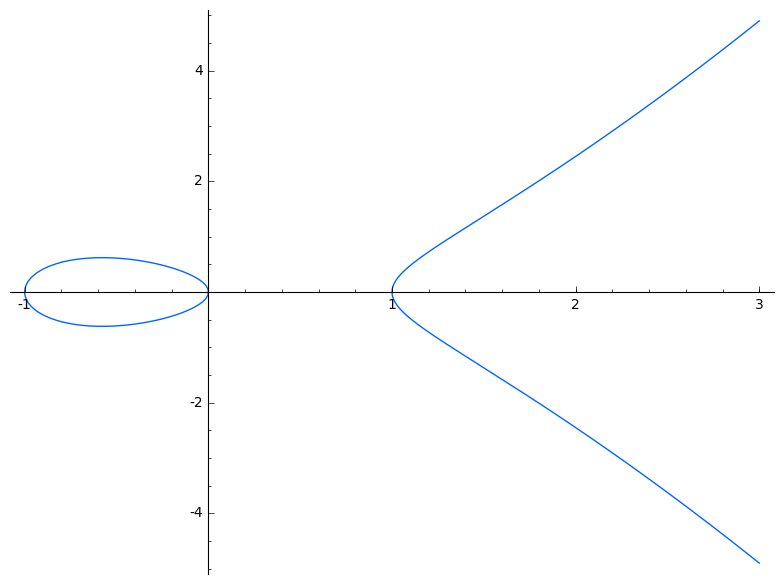
\includegraphics[width=0.5\textwidth]{ej1}
    \caption{Salida Código \ref{cod:ej1}}
    \label{fig:ej1}
\end{figure}

Programamos de forma similar el código para visualizar la gráfica de la curva dada por la ecuación $y^2=x^3+x$, véase el Código \ref{cod:ej2}, cuya salida se encuentra en la Figura \ref{fig:ej2}

\begin{lstlisting}[label={cod:ej2}, caption={Curva elíptica $y^2=x^3+x$}, morekeywords={sage}]
sage: E =  EllipticCurve(RR, [1, 0]);
      plot(E, (-2, 4), color=hue(0.8))
\end{lstlisting}

\begin{figure}[H]
    \centering
    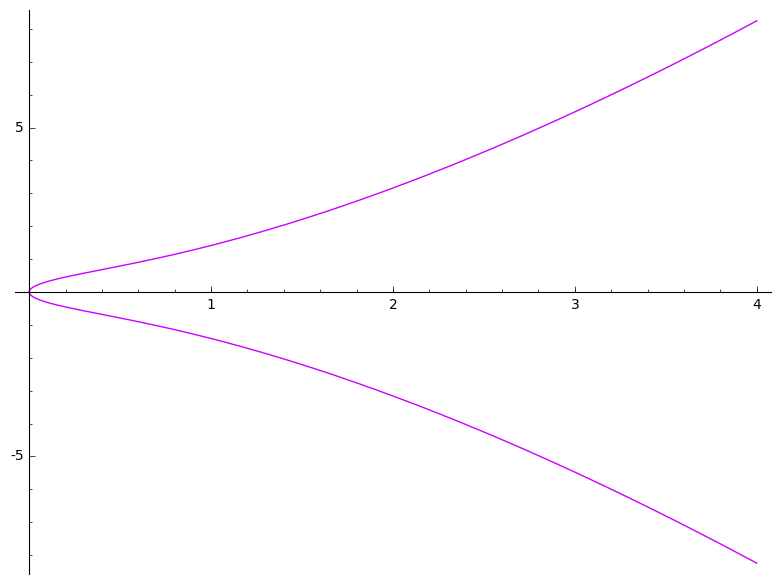
\includegraphics[width=0.5\textwidth]{ej2}
    \caption{Salida Código \ref{cod:ej2}}
    \label{fig:ej2}
\end{figure}

En la Figura \ref{fig:EllipticCurveCatalog} tenemos una tabla con la forma de las curvas elípticas para valores enteros de $a$ entre -2 y 1 y $b$ entre -1 y 2.

\begin{figure}[H]
    \centering
    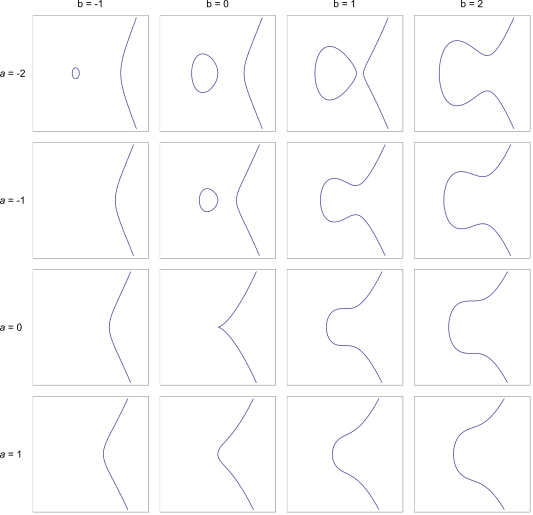
\includegraphics[width=0.7\textwidth]{EllipticCurveCatalog}
    \caption{Ejemplos de curvas elípticas}
    \label{fig:EllipticCurveCatalog}
\end{figure}



\subsection{Estructura de grupo}
Dada una curva elíptica podemos definir un grupo abeliano formado por puntos de la misma. 
\begin{enumerate}
\item Tomamos como elemento neutro el punto del infinito $ \{\infty\} $.
\item El opuesto de un punto $ P $ viene dado por su simétrico por el eje $ X $. Más concretamente, si $ P = (x_P, y_P) $ entonces $ -P = (x_P, -y_P) $.
\item En general, dados dos puntos de la curva $ P = (x_P, y_P) $ y $ Q = (x_Q, y_Q) $ con $ x_P \neq y_P $, su suma es el punto $ -R $ que viene definida por:
\[
(x_R, -y_R) =(m^2 − x_P − x_Q, -y_P - m(x_R − x_P )) = (m^2 − x_P − x_Q, -y_Q - m(x_R − x_Q )),
\]
donde
\[
m = \frac{y_P-y_Q}{x_P-x_Q}.
\]
Puede causar asombro que definamos $ P+Q=-R $. Esto se deba al sentido geométrico de la suma en la curva. Esta operación debe seguir la siguiente regla: ``dados tres puntos $ P$, $ Q $ y $ R $ alineados y no nulos su suma $ P + Q + R $ debe ser el elemento neutro''. Por lo tanto, $ P +Q $ es el opuesto al punto de corte de la recta que une ambos puntos. De ahí también notamos la presencia del signo menos en la segunda coordenada tal y como indicamos en el punto anterior. También notar que el sentido geométrico nos aporta intuitivamente la conmutatividad ya que la recta tangente es la misma en el caso $ P+Q $ y $ Q+P $ y la asociatividad ya que $ (P+Q) + R = P + (Q+R) = (P+R) + Q$ (y las demás posibilidades).\\

No podemos usar estas fórmulas en algunos casos especiales, poe ejemplo cuando $ P=Q $. En este caso no existe una sola recta que pase por ``ambos'' puntos. Sin embargo, si nos aproximamos a $ Q $ mediante puntos $ Q' $ con $ Q' \neq P $ en seguida vemos que la recta que obtendríamos es la tangente en $ P $. Así, definimos su suma como el opuesto del punto de intersección de la recta tangente en $ P $. Otra situación interesante es cuando $ P \neq Q $ pero no hay más puntos de corte. Nos encontramos en un caso parecido al anterior ya que uno de los puntos es tangente a la curva. Si suponemos que $ P $ es donde se da la tangencia, por el caso anterior tememos que $ P + P = -Q $ por lo que $ P + Q = -P $. En estas situaciones de tangencia tenemos que:
\[
m = \frac{3x^{2}_P + a}{2y_P}.
\]
En ambos casos debemos comprobar que la suma pertenece a la curva y que los tres puntos están alineados.

\item Finalmente, dado $ n \in \mathbb{Z} $, el producto por escalares lo definimos como:
\[   
nP = 
\begin{cases}
 (P+\stackrel{n}{\cdots}+P) &\text{si } n > 0\\
0 &\text{si } n = 0\\
(-P\stackrel{n}{\cdots}-P) &\text{si } n < 0\\
\end{cases}
\]
\end{enumerate}

%---lo necesito para la parte de ECDSA sino se usa en otro sitio ponerlo en ECDSA
Parámetros de dominio para los algoritmos (p, a, b, G, n, h) donde:
\begin{itemize}
	\item p: primo
	\item a, b: Coeficientes de la curva elíptica, hay que elegirlos con cuidado para que el algoritmo sea seguro
	\item G: Generador del grupo
	\item n: Orden del grupo
	\item h: Cofactor del subgrupo
\end{itemize}
%----
\subsection{El problema del logaritmo discreto}
La seguridad de la criptografía de la curva elíptica reside en la dificultad para calcular logaritmos discretos. Este problema es análogo el de otros criptosistemas como el Digital Signatura Algorithm (DSA) o el intercambio de llaves mediante el mecanismo de Diffie-Hellman.

En nuestro caso, el problema consiste en lo siguiente: ``si conocemos $ P $ y $ Q $ dos puntos de la curva elíptica, ?`podemos encontrar un $ k $ tal que $ Q = kP $? ''. Vemos que no estamos calculando un logaritmo como tal pero se sigue usando ese término por analogía a otros sistemas como se ha mencionado anteriormente. 

Actualmente, no existe ninguna demostración matemática que efectivamente pruebe la dificultad de dicho cálculo. Solo sabemos que es difícil pero no podemos estar seguros. Con el siguiente ejemplo ilustramos su complejidad. Para ello usamos un algoritmo ``Baby-step, giant-step'' que se basa en el hecho de que cualquier entero $ x $ puede expresar como $ x = am+b $ con $ a,m \text{ y } b$ también enteros. Escribimos entonces:
\begin{equation*}
\begin{split}
Q &= xP \\
  &= (am+b)P\\
  &=amP + bP.
\end{split}
\end{equation*}
Así, podemos expresar $ Q - amP  = bP $. El algoritmo consiste en en calcular algunos valores de $ bP $ y otros de $ Q-amP $ hasta que encontremos una correspondencia. El algoritmo también indica que debemos escoger $ m = \sqrt{n} $ y los números $ a $ y $ b $ se mueven entre 0 y $ m $ por lo que mientras $ bP $ tiene incrementos pequeños (``baby'') $ amP $ los tiene grandes (``huge''). Este método nos aporta una complejidad tanto en tiempo como en memoria de $ O(\sqrt{n}) $ . Este ataque tiene entonces complejidad exponencial pero es mejor que uno de fuerza bruta. De todos modos sigue siendo intratable ya que para un $  n  $ tal que $ \sqrt{n} = 7.922816251426434 \times 10^{28} $ el almacenamiento de datos que podemos llegar a necesitar es de $ 2,5\times10^{30} $ bytes de memoria (la capacidad de almacenamiento mundial es de aproximadamente $ 10^{21} $ bytes).

\section{Algoritmos}

\subsection{ECDSA}

ECDSA es un algoritmo de firma digital, Elliptic Curve Digital Signature Algorithm, es una variante del algoritmo DSA (Digital Signature Algortihm) aplicado a curvas elípticas. Trabaja con el hash del mensaje en lugar de con el propio mensaje. La elección de la función hash es importante, de esto dependerá la seguridad del sistema criptográfico. El hash del mensaje tendrá una longitud de \textit{n} bit.

Imaginemos que Alice quiere firmar un mensaje con su llave privada ($d_{A}$), y la otra persona, Bob, quiere validar la firma con la llave pública de Alice ($H_{A}$). Alice es la única que puede producir las firmas válidas, sin embargo todo el mundo que tenga su llave pública puede verificarlas.

Alice y Bob están usando los parámetros del dominio. El hash truncado lo denotaremos por \textit{z}.

\subsubsection*{Firma del mensaje}
Algoritmo de firma del mensaje de Alice, a partir de \textit{k} y \textit{z} se genera la firma con la clave privada de Alice:


\begin{enumerate}
	\item Tomamos un entero k de forma aleatorio en el conjunto \{ 1, ..., n-1\}.
	\item Calcular \textit{P} = \textit{kG}.
	\item Calcular el número \textit{r = $x_{P}$}.
	\item Si \textit{r} es 0 entonces se toma otro \textit{k} y se intenta de nuevo.
	\item Se calcula \textit{s} = \textit{$k^{-1}$}(\textit{z} + \textit{r$d_{A}$}) mod \textit{n}  con \textit{$k^{-1}$} el inverso multiplicativo de \textit{k} módulo \textit{n}.
	\item Si \textit{s} es 0 entonces se elige otro \textit{k} y se vuelve al principio.
\end{enumerate} 

Al final obtendremos la firma que será la pareja (\textit{r}, \textit{s}) 


Si el subgrupo tiene orden no primo, entonces el algoritmo ECDSA no se puede usar.

\subsubsection*{Verificación de la firma}
Ahora entra en juego Bob que para validar la firma, a partir del mensaje firmado y de \textit{z} con la clave pública de Alice \textit{$H_A$}.

\begin{enumerate}
	\item Calcular \textit{$u_1$} = \textit{$s^{-1}$ z} mod\textit{n}
	\item Calcular \textit{$u_2$} = \textit{$s^{-1}$ r} mod\textit{n}
	\item Calcular el punto \textit{P} = \textit{$u_1$G} + \textit{$u_2$$H_A$}	
\end{enumerate}

La firma solo es válida si \textit{r} = \textit{$x_P$} mod\textit{n}


\subsubsection*{Exactitud del algoritmo}
Veamos que esta definición de \textit{P} del punto 3 con la definición anterior de \textit{P} = \textit{kG}

Partimos de \textit{P} = \textit{$u_1$G} + \textit{$u_2$$H_A$}, sustituimos el valor de la clave pública \textit{$H_A$} = \textit{$d_A$G}


\begin{align}
\begin{split}
\textit{P} &= \textit{$u_1$G} + \textit{$u_2$$H_A$}\\ &= \textit{$u_1$G} + \textit{$u_2$$d_A$G}\\
&= (\textit{$u_1$} + \textit{$u_2$$d_A$})\textit{G}\\
\end{split}
\end{align}

Sustituimos los valores de $u_1$ y $u_2$ que hemos declarado en la verificación de la firma:

\begin{align}
\begin{split}
P &= (\textit{$u_1$} + \textit{$u_2$$d_A$})\textit{G}\\
&= (\textit{$s^{-1}$z} + \textit{$s^{-1}$r$d_A$}) \textit{G}\\
&= \textit{$s^{-1}$}(\textit{z} + \textit{r$d_A$}) \textit{G}\\
\end{split}
\end{align}

Como el subgrupo cíclico de orden \textit{n} en el que estamos trabajando está generado por \textit{G} por tanto no hace falta poner ``mod \textit{n}'' si múltiplicamos por \textit{G}.


Ahora nos fijamos en la definición de \textit{s} = \textit{$k^{-1}$}(\textit{z} + \textit{r$d_A$}) mod \textit{n}. Multiplicamos por \textit{k} a ambos lados y dividimos por \textit{s} y obtenemos: \textit{k} = \textit{$s^{-1}$}(\textit{z} + \textit{r$d_A$}) mod \textit{n}

\begin{align}
\begin{split}
P &= \textit{$s^{-1}$}(\textit{z} + \textit{r$d_A$}) \textit{G}\\
&= \textit{kG}
\end{split}
\end{align}


\subsubsection*{Importancia de \textit{k}}

Es importante el valor que escojamos de \textit{k} la clave secreta. Si además siempre firmamos con el mismo valor de \textit{k} y con los mismos valores aleatorios, para los atacantes serían más fácil encontrar la clave privada.

Para descubrir la clave privada \textit{$d_S$} necesitamos calcular \textit{k} a partir de los hashes \textit{$z_1$} y \textit{$z_2$} y de las correspondientes firmas (\textit{$r_1$}, \textit{$s_1$}) y (\textit{$r_2$}, \textit{$s_2$})


\begin{enumerate}
	\item $r_1$ es igual a $r_2$, puesto que \textit{r} = \textit{$x_P$} mod \textit{n} y \textit{P} = \textit{kG} es el mismo para las dos firmas.
	\item Observamos que  (\textit{$s_1$} - \textit{$s_2$}) mod\textit{n} = \textit{$k^{-1}$} (\textit{$z_1$} - \textit{$z_2$}) mod\textit{n} viene directamente de la definición de \textit{s}
	\item \textit{k}(\textit{$s_1$} - \textit{$s_2$}) mod\textit{n} = (\textit{$z_1$} - \textit{$z_2$}) mod\textit{n}
	\item \textit{k}  = (\textit{$z_1$} - \textit{$z_2$}) $(\textit{$s_1$} - \textit{$s_2$})^{-1}$ mod\textit{n}
\end{enumerate}

Ahora despejamos \textit{$d_S$} de la definición de \textit{s} y obtenemos que:


\begin{align}
\begin{split}
\textit{s} &= \textit{$k^{-1}$}(\textit{z} + \textit{r$d_S$}) mod \textit{n}\\
\textit{$d_S$} &= \textit{$r^{-1}$}(\textit{sk} - \textit{z}) mod \textit{n}\\
\end{split}
\end{align}

Así hemos conseguido la clave privada con los valores que conocemos.

\subsection{ECDH}

\subsection{Comparación con RSA}

La principal diferencia entre la criptografía de la curva elíptica y la de RSA, es la cantidad de almacenamiento que se necesita para guardar una clave al mismo nivel de seguridad. Por ejemplo, si para guardar una clave de RSA se necesitan 1024 bits, para almacenar la de ECC se requiere de 160, las diferencias son aún mayores cuando aumenta el nivel de seguridad, para RSA son necesarios 15360 bits mientras que para ECC son 521 bits.

La relación entre los tamaños no es lineal, es decir, si multiplicamos por \textit{k} el tamaño de RSA, no tenemos \textit{k} veces el tamaño de ECC.

Por otro lado, la generación de la clave y la firma es considerablemente más rápido con ECC que con RSA.


Los algoritmos más rápidos para el computo de logaritmos discreots, además de la curva elíptica, son Pollard's rho y baby-step giant-step. Destaca uno en particula que es el algoritmo ``criba general del cuerpo de números'' el más rápido conocido a día de hoy para la factorización de enteros, que además se puede usar para el logaritmo discreto.


\section{Conclusiones}




%Apéndice
\appendix
\renewcommand{\thesection}{\Roman{section}}
\setcounter{section}{0}
\section{Glosario}



\end{document}
